\chapter{Proposed Changes to the Protocol Design}\label{ch:protocol-changes}

For a definition of the \drivel{} protocol, as we implemented it in the course of this thesis, we refer readers to \cref{fig:drivel}, which served as our primary source.
This section dives into a theoretical discussion of proposed improvements to the protocol to better support traffic shaping and improve memory performance and suggests alternatives to \cref{fig:drivel}.
Future implementations may want to take inspiration from the ideas presented here to further improve \drivel{}.

\section{Discussion on Fragmenting Handshake Messages} \label{ssec:fragmentation}

This section analyzes possibilities to allow for more flexibility in shaping \drivel{} traffic. Avoiding fingerprinting based on certain sizes, directionalities and timing of messages between client and bridge is crucial to evade censors.

\textbf{No changes discussed or proposed in this \cref{ssec:fragmentation} were implemented, or practically evaluated as part of this thesis, but this discussion may be valuable to readers to understand possible future directions of the protocol.}

\paragraph{Fragmentation is Needed}
When deploying \drivel{}, it may be desirable to offer even more flexibility for traffic shaping than \obfsfour{}. In particular, \obfsfour{} sends two messages in its handshake, before fragmenting packets using a customizable message size distribution based on a deterministic pseudorandom number generator and a seed determined by the bridge server.

While \drivel{} also requires two messages to complete the handshake, \obfsfour{} messages range from 141 to 8 192 bytes in length, and \drivel{} message sizes depend on the selected KEM and OKEM. Ignoring the padding for the moment, \cref{tab:frag-msg-sizes} gives an overview of the minimum message sizes required for different combinations of KEM and OKEM in \drivel{}.

\begin{table}
    \centering \footnotesize
    \begin{tabular}{@{} L{0.2\textwidth-\tabcolsep} L{0.33\textwidth-2\tabcolsep} | L{0.3\textwidth-\tabcolsep} @{}}
    KEM with\newline Parameter Sets & OKEM with\newline Parameter Sets & Minimum Sizes (bytes)\newline Level 1 / Level 3 / Level 5 \\ \hline
    
    \multirow{4}{*}[-2.6em]{\shortstack[l]{ML-KEM\\ 512 / 768 / 1024}}
    & Classic-McEliece\newline 348864 / 460896 / 6688128\vspace{0.3em} & 928 / 1 372 / 1 808 \\
    & ML-Kemeleon\newline 512 / 768 / 1024\vspace{0.3em} & 1 709 / 2 468 / 3 258 \\
    & FEO-HQC\newline 128 / 192 / 256\vspace{0.3em} & 5 265 / 10 194 / 16 021 \\
    & FrodoKEM\newline 640 / 976 / 1344\vspace{0.3em} & 10 552 / 16 960 / 23 232 \\ \hline

    \multirow{4}{*}[-2.6em]{\shortstack[l]{BIKE\\ L1 / L3 / L5}}
    & Classic-McEliece\newline 348864 / 460896 / 6688128\vspace{0.3em} & 1 669 / 3 271 / 5 362 \\
    & ML-Kemeleon\newline 512 / 768 / 1024\vspace{0.3em} & 2 450 / 4 367 / 6 812 \\
    & FEO-HQC\newline 128 / 192 / 256\vspace{0.3em} & 6 006 / 12 093 / 19 575 \\
    & FrodoKEM\newline 640 / 976 / 1344\vspace{0.3em} & 11 293 / 18 859 / 26 786 \\ \hline

    \multirow{4}{*}[-2.6em]{\shortstack[l]{HQC\\ 128 / 192 / 256}}
    & Classic-McEliece\newline 348864 / 460896 / 6688128\vspace{0.3em} & 2 377 / 4 710 / 7 485 \\
    & ML-Kemeleon\newline 512 / 768 / 1024\vspace{0.3em} & 3 158 / 5 806 / 8 935 \\
    & FEO-HQC\newline 128 / 192 / 256\vspace{0.3em} & 6 714 / 13 532 / 21 698 \\
    & FrodoKEM\newline 640 / 976 / 1344\vspace{0.3em} & 12 001 / 20 298 / 28 909 \\ \hline

    \multirow{4}{*}[-2.6em]{\shortstack[l]{FrodoKEM\\ 640 / 976 / 1344}} 
    & Classic-McEliece\newline 348864 / 460896 / 6688128\vspace{0.3em} & 9 744 / 15 820 / 21 760 \\
    & ML-Kemeleon\newline 512 / 768 / 1024\vspace{0.3em} & 10 525 / 16 916 / 23 210 \\
    & FEO-HQC\newline 128 / 192 / 256\vspace{0.3em} & 14 081 / 24 642 / 35 973 \\
    & FrodoKEM\newline 640 / 976 / 1344\vspace{0.3em} & 19 368 / 31 408 / 43 184
    \end{tabular}
    \caption[
        Minimum sizes in bytes for the first \drivel{} message without padding depending on the choice of KEM and OKEM
    ]{
        Minimum sizes in bytes for the first \drivel{} message without padding depending on the choice of KEM and OKEM. Each cell contains minimum sizes for NIST security levels 1, 3, and 5.
        In the case of Classic McEliece, specific KEM parameter sets were selected to minimize message sizes while maintaining the targeted security level. The KEM parameter sets are identified in the first two columns.
    }
    \label{tab:frag-msg-sizes}
\end{table}

The concern in this section is that censors may observe particular traffic patterns. In particular, a bridge server never sends a reply before receiving the entire first \drivel{} or \obfsfour{} message in order to avoid probing attacks. This leads to quiet periods which may constitute an identifiable feature of the pluggable transport.

As is obvious from the table, sending the entire first \drivel{} message in full before the bridge responds (after verifying the PRF value at the end of message) leads to a large quiet period. Thus, for all but a few KEM/OKEM combinations, this quiet period would quickly be identifiable. At best, using Classic McEliece or ML-Kemeleon as an OKEM while employing ML-KEM or BIKE as a KEM still yields sizes not exceeding 8 192 bytes but the quiet periods would still be easy to distinguish from e.g.~\obfsfour{} traffic.

\paragraph{Desirable Security Properties}
Before discussing the options to mitigate this risk, let us recall one of the advantages \drivel{} has over \obfsfour{}. In \obfsfour{}, censors can retroactively identify handshake packets by verifying the MAC value if the bridge information is leaked, as the MAC it is keyed only with the bridge information. This allows censors to definitively identify clients that had previously connected to a bridge, as well as any future clients connecting to the bridge. This property has been discussed in \cite[Section~6]{CCS:GunSteVei24} and was also recognized earlier by David Fifield in \cite{obfs4-pk-reveal-distinguisher}.

Instead, \drivel{} establishes a shared secret between the client and the bridge in the first message. This shared secret is then used in addition to the bridge information to key the PRF. Censors therefore cannot retroactively identify obfuscated key exchanges with certainty, unless the OKEM private key is leaked. We will refer to this property here as \emph{strong obfuscation} ($\sObf$), as formally defined in \cite{CCS:GunSteVei24}.

For $\drivel$ to maintain its security, it is necessary that:
\begin{itemize}
    \item[a)] the bridge verifies the client's knowledge of the bridge information before sending a reply, and that
    \item[b)] the client's message proving this is indistinguishable from random bits, even given the bridge information and independent proofs from other clients.
\end{itemize}

Violating a) would make the bridge vulnerable to probing attacks by censors that do not know the bridge information. On the other hand, violating b) would trivially break $\sObf$. Both of these outcomes would be undesirable and $\sObfKE$ from \cite{CCS:GunSteVei24} captures both avenues of attack, since the predicate \textsf{Probed} automatically wins the game, and public keys can be revealed when asked to distinguish a simulated from a real transcript in \textsc{ChallExec}, respectively.

Due to the required proof in the client's initial communication alone, it is strictly necessary that the bridge server receive a certain minimum amount of data before it may respond in any way.
To break up the first large \drivel{} message, we could, for example, split it into parts and let the server respond after receiving smaller parts. However, the first such ``fragment'' would need to contain at least a suitable proof that the client knows the bridge information.

\paragraph{An Informal Security Notion}
In order to outline the above requirements a bit more, we can informally define the initial interaction between an adversary and the bridge servers. One goal of the initial exchange, among others, is to arrive at a shared secret, that can aid in subsequent fragmentation, using just the first message from the client to the server.

This effectively means that a first fragment could be viewed as an (O)KEM ciphertext: Some bridge information is generated and distributed (similar to a public key), a message is sent by a client to the bridge and a shared secret is computed from it.
% Conversely, the first fragment may also be viewed as a MAC tag: Bridge information is then assumed to be secret and shared between two parties (similar to a symmetric key), and used to authenticate a communication.

Let us also assume that there is no possibility for bridges to save state about each client, that clients are unwilling to save state for the bridges due to privacy concerns (both options could be implemented e.g. similar to TLS 1.3 session resumption \cite[Section~2.2]{rfc8446}) and that no pre-shared symmetric keys are available (which would trivialize the entire handshake).

For the following discussion, let $P$ be the bridge information.
Let $M$ denote the fixed-length message sent from the client to the bridge, and let $S$ denote the shared secret computed by both client and bridge for the secure transport of subsequent traffic.
% We also define two adversaries $\adv$ and $\bdv$. The bridge information $P$ is only known to $\adv$, and not $\bdv$.
We also define an adversary $\adv$, to which the bridge information $P$ is known.
The goal of $\adv$ is to identify traffic as a client-bridge handshake (breaking strong obfuscation).
% and $\bdv$ attempts to elicit a response from a bridge (breaking probing resistance).

We will now examine what properties (in addition to probing resistance) this exchange should satisfy:
\begin{itemize}
    \item The adversary $\adv$ should not be able to distinguish the first fragment sent over the network from random bits, even given $P$ (e.g. retroactively). This corresponds directly to $\ctxtunif$, if we were to view the exchange as an OKEM.

    \item The adversary $\adv$ should not be able to distinguish a randomly sampled shared secret $S$ from one corresponding to any given message $M$ observed on the network, even if the adversary is allowed further communication with the bridge. Viewing the exchange as a KEM, this corresponds to $\indcca$ security.
    
    % \item The adversary $\bdv$ should not be able to create a message $M$ that, when parsed by the bridge results in a valid shared secret $S$ without access to the bridge information. This would allow bridges to respond, violating probing resistance. Instead, the bridge should reject the message. Here, we can view the exchange as a MAC application using the previously shared bridge information $P$ as a key. The property then corresponds to the standard notion of strongly secure MACs as defined in \cite[Definition~4.3]{katz_lindell}, \cite[Chapter~2]{AC:BelNam00}.
\end{itemize}

Note also that in the case of \drivel{}, without any modifications discussed below, these properties are achieved when choosing $M$ to be the entire first protocol message:
% The first two requirements are covered by the OKEM, and the last property is achieved by authenticating every message with a PRF value.
The OKEM covers both requirements, and probing resistance is also achieved by authenticating every message with a PRF value.

It is hard to imagine a significant potential in message size reduction outside of removing other components of the first \drivel{} message, as we conjecture the following:
Any protocol satisfying the requirements listed above could act as an OKEM.
%(or an inefficient MAC).
The existence of a more efficient protocol would thus imply the existence of a more efficient OKEM, which, due to the large scope of the NIST Standardization, seems implausible.
This gives us confidence that the constructions in \cref{ssec:drivel-mod} below are both close to optimal in terms of the size of the first fragment.

\paragraph{Arbitrary Fragmentation}
We have focused on maintaining $\sObf$ security during fragmentation up until now, as this was also a design goal for \drivel{}.
If, however, compromises could be made in regards to $\sObf$ security, the fragmentation would not suffer the constraints outlined above.

Relaxing our requirements, and allowing a censor to retroactively identify bridges given their bridge information, the following fragmentation strategy becomes reasonable: The client sends a first fragment of $x+16$ bytes, consisting only of $x$ bytes of uniformly random data and a 16 byte PRF keyed with the bridge information. Padding may be added between the two blocks. The choice of $x$ does not impact the security, but reduces the chance of bridges rejecting honest connection attempts due to repeated PRF values.

The rejection of repeated PRF values works using ``epoch hours'', i.e. the number of seconds since the Unix epoch divided by 60.
The current epoch hour is used as an input to every PRF calculation, and verifiers only accept PRF values that used an epoch hour not different from their local value by more than 1.
This allows bridges to partially clear the set of already received PRF values (used to prevent replay attacks checks) every hour.
In particular, the value of $x$ must be such that the chance of collisions in those $x$ bytes must be kept small within a given epoch hour.

As an example, \cite{tor-metrics} reports around 112 000 users across all pluggable transports and around 1 900 bridges, so assuming an even distribution of users across bridges, this would mean an average of 60 active users per bridge, each making at most 60 handshakes per epoch hour. Using those numbers, choosing $x=6$ already yields a collision probability $\leq 3 \cdot 10^{-8}$ by the birthday bound (with $2^{48}$ possible values and only $2^{11.8}$ samples per epoch hour).

This approach is very similar in spirit to the first message in \obfsfour{} (in that it does not use a shared secret in the calculation of the PRF value) and allows for much more flexibility in traffic shaping through padding. The key difference from \obfsfour{} is the removal of one of the PRF values and the aggressive reduction in message size by replacing the obfuscated client public key with randomized data.

If implementations are willing to accept some additional complexity, these $x$ bytes of uniformly random data might also be replaced with the start of any key exchange message that would be sent after this initial message (e.g. the first $x$ bytes of $\mathsf{epk}_e$ in the case of \drivel{}). This would achieve the same effect of proving that the client knows the bridge information as soon as possible, as long as collisions in the first $x$ bytes are sufficiently unlikely.

Sending even less data in a first fragment seems implausible, as the randomized data is necessary to prevent replay attacks while avoiding false positives, and the PRF value proves knowledge of the bridge information. Using less than $x$ or 16 bytes, respectively, for either component would lower the security level or increase the collision probability between users, forcing handshake retries.

\section{Proposed Modifications to the Drivel Protocol} \label{ssec:drivel-mod}

No changes discussed or proposed in this \cref{ssec:drivel-mod} were implemented or practically evaluated as part of this thesis, but this discussion may be valuable to readers to understand possible future directions of the protocol.

This thesis employs only the unmodified variant of $\drivel{}$ presented in \cref{fig:drivel}.

The following two subsections offer different approaches to implement fragmentation of handshake messages in \drivel{}. \Cref{sssec:variant-minimal} tries to make only small changes to \drivel{}, as proposed in \cref{fig:drivel}, while \cref{sssec:variant-framing} tries to reuse existing mechanisms in \obfsfour{} and extend them from the data transfer to the handshake phase.

\subsection{Variant 1: A Minimal Fragmentation} \label{sssec:variant-minimal}

One way to achieve the security properties described in \cref{ssec:fragmentation} in a space-efficient manner would be to send one OKEM ciphertext plus a 16 byte PRF value as the first fragment. The PRF would be keyed by a combination of the shared secret and the bridge information (as in \drivel{}).

Recall from \cref{fig:drivel} that the first \drivel{} message is constructed as $\mathsf{epk}_e \conc c_S \conc P_C \conc M_C \conc \mathsf{MAC}_C$, where $\mathsf{epk}_e$ is the encrypted KEM public key, $c_S$ is the OKEM ciphertext of interest, $M_C$ helps delimit the message, and $\mathsf{MAC}_C$ authenticates all preceding data.

In this fragmentation approach, we propose a minimal change to this message, such that encrypted public keys $\mathsf{epk}_e$ are sent later, and an additional PRF value (the ``authenticator'') is sent directly following the OKEM ciphertext. Reusing the same variables, parenthesizing the first fragment for clarity, and introducing $A_C \gets F_1(ES, c_S \conc \text{``:authc''})$ as an authenticator, this would lead to the following first protocol message:

\[
    \left( c_S \conc A_C \right) \conc \mathsf{epk}_e \conc P_C \conc M_C \conc \mathsf{MAC}_C .
\]

Using this modified first message, the bridge may now start sending data earlier than in unmodified \drivel{}. Although it cannot send its second message before receiving $\mathsf{epk}_e$, it can send dummy data that the client will ignore.

The adapted protocol specification is visualized in \cref{fig:modified-drivel-minimal}, an adaptation of \cref{fig:drivel}. Dashed lines denote the option to send dummy data for the purpose of traffic shaping.

\begin{figure}
    % \begin{minipage}[t]{\textwidth}
	\hfill
	\pseudocode[codesize=\footnotesize,jot=-1mm]{%
		\textbf{Server key generation/setup} \\
		\nodeid \getsr \bin^{\nodeidlen} \\
		(\pk_S, \sk_S) \getsr \OKEM.\kgen() \\
		\pstate.\macregister \gets \emptyset \\
		\text{return } ((\pk_S, \nodeid), (\sk_S, \nodeid), \pstate)
	}
	\hspace*{0.8cm}
% \end{minipage}

% \vspace{0.5em}

% \hspace*{-0.2in}
\centering
\scalebox{0.77}{%
\begin{tikzpicture}
	% Set the X coordinates of the client, server, and arrows
	\edef\ClientX{0}

	\edef\ArrowLeft{3}
	\edef\ArrowRight{13}
	\edef\ServerX{16.5}
	\edef\ServerLeftTextwidth{10.5cm} % width of server-side text, when left-aligned

	% Set the starting Y coordinate
	\edef\Y{0}

	% Draw header boxes
	\node [rectangle,draw,inner sep=5pt,right] at (\ClientX,\Y) {\textbf{Client}};
	\node [rectangle,draw,inner sep=5pt,left] at (\ServerX,\Y) {\textbf{Server}};
	
	\NextLine[0.4]
	\ClientAction[gray,font=\small]{\hspace{1.5cm}knows $(\pk_S, \nodeid)$}
	\ServerAction[gray,font=\small]{knows $(\sk_S, \nodeid)$\hspace{1.5cm}\null}
	\NextLine[1.1]
	
	\ClientAction{$(\pk_e, \sk_e) \getsr \KEM.\kgen()$} 
	\NextLine
	\ClientAction{$P_C \getsr \mathcal{D}_{\mathsf{pad}_C}$}
	\NextLine
	\ClientAction{$(c_S, K_S) \getsr \OKEM.\encaps(\pk_S)$}
	\NextLine
	\ClientAction{$ES \gets \funComb(\nodeid, K_S)$}
	\NextLine
	\ClientAction{$EK_1 \gets \funPRF(ES, \textlit{:enckey1}, \keylen_1)$}
	\NextLine
	\ClientAction{$EK_2 \gets \funPRF(ES, \textlit{:enckey2}, \keylen_2)$}
	\NextLine
	\ClientAction{$\mathsf{epk}_e \gets \funEnc(EK_1, \pk_e)$}
	\NextLine
	\ClientAction{\highlightbox{$A_C \gets \funPRF(ES, c_S \conc \textlit{:authc})$}}
    \NextLine
	\ClientAction{\highlightbox{$A_S \gets \funPRF(ES, \textlit{:auths})$}}
	\NextLine
	\ClientAction{$M_C \gets \funPRF(ES, \mathsf{epk}_e \conc \textlit{:mc})$}
	\NextLine
	\ClientAction{$\mathsf{MAC}_C \gets \funPRF(ES,$\highlightbox{$c_S \conc A_C \conc \mathsf{epk}_e$}$\conc P_C \conc M_C \conc \textlit{:mac\_c})$}
	%%%%%%%%%%%%%%%%%%%%%%%%%%%%%%%%%%%%%%%%%%%%%%%%%%%%%%%%%%%%%%%%%%%%%%%%%%%%%%%%%%%%%%%%%%%%%%%%%%%%%%%
	\NextLine[2]
	\ClientToServer{\highlightbox{$\mathsf{msg}_C' = c_S \conc A_C$}}{}
	\NextLine
    %%%%%%%%%%%%%%%%%%%%%%%%%%%%%%%%%%%%%%%%%%%%%%%%%%%%%%%%%%%%%%%%%%%%%%%%%%%%%%%%%%%%%%%%%%%%%%%%%%%%%%%

    % Server verifies A_C and can start with dummy data
    \ServerActionLeft{$c_S \gets \mathsf{msg}_C'[1..\obfctxtlen]$ ; \highlightbox{$A_C \gets \mathsf{msg}_C'[\obfctxtlen+1..\obfctxtlen+\funPRFoutlen]$}}
	\NextLine
	\ServerActionLeft{$K_S \gets \OKEM.\decaps(\sk_S, c_S)$}
	\NextLine
	\ServerActionLeft{$ES \gets \funComb(\nodeid, K_S)$}
	\NextLine
	\ServerActionLeft{$EK_1 \gets \funPRF(ES, \textlit{:enckey1}, \keylen_1)$}
	\NextLine
	\ServerActionLeft{$EK_2 \gets \funPRF(ES, \textlit{:enckey2}, \keylen_2)$}
	\NextLine
	\ServerActionLeft{\highlightbox{if $\funPRF(ES, c_S \conc \textlit{:authc}) \neq A_C$: $\texttt{break}$}}
	\NextLine
	\ServerActionLeft{if \highlightbox{$A_C$}$ \in \pstate.\macregister$: $\texttt{break}$}
	\NextLine
	\ServerActionLeft{$\pstate.\macregister \gets \pstate.\macregister \cup $\highlightbox{$\{A_C\}$}}
    \NextLine
	\ServerActionLeft{\highlightbox{$A_S \gets \funPRF(ES, \textlit{:auths})$}}
    %%%%%%%%%%%%%%%%%%%%%%%%%%%%%%%%%%%%%%%%%%%%%%%%%%%%%%%%%%%%%%%%%%%%%%%%%%%%%%%%%%%%%%%%%%%%%%%%%%%%%%%
    \NextLine[0.5]
	\ServerToClient[dashed,->]{}{}
	%%%%%%%%%%%%%%%%%%%%%%%%%%%%%%%%%%%%%%%%%%%%%%%%%%%%%%%%%%%%%%%%%%%%%%%%%%%%%%%%%%%%%%%%%%%%%%%%%%%%%%%

    % Client waits for A_S
	\ServerAction{\highlightbox{send arbitrary data}}
    \ClientAction{\highlightbox{discard until $A_S$}}
    %%%%%%%%%%%%%%%%%%%%%%%%%%%%%%%%%%%%%%%%%%%%%%%%%%%%%%%%%%%%%%%%%%%%%%%%%%%%%%%%%%%%%%%%%%%%%%%%%%%%%%%
    \NextLine[1.2]
	\ClientToServer{$\mathsf{msg}_C'' = $\highlightbox{$\mathsf{epk}_e \conc P_C$}$ \conc M_C \conc \mathsf{MAC}_C$}{}
	\NextLine
	%%%%%%%%%%%%%%%%%%%%%%%%%%%%%%%%%%%%%%%%%%%%%%%%%%%%%%%%%%%%%%%%%%%%%%%%%%%%%%%%%%%%%%%%%%%%%%%%%%%%%%%

    % Server parses rest of message and replies
    \ServerActionLeft{$\mathsf{epk}_e \gets \mathsf{msg}_C''[1..\pklen]$}
	\NextLine
	\ServerActionLeft{$M_C \gets \funPRF(ES, \mathsf{epk}_e \conc \textlit{:mc})$}
	\NextLine
	\ServerActionLeft{parse $(\mathsf{epk}_e \conc P_C \conc M_C \conc \mathsf{MAC}_C) \gets \mathsf{msg}_C''$ using $M_C$; else $\texttt{break}$}
	\NextLine
	\ServerActionLeft{if $\funPRF(ES,$\highlightbox{$c_S \conc A_C \conc \mathsf{epk}_e$}$\conc P_C \conc M_C \conc \textlit{:mac\_c}) \neq \mathsf{MAC}_C$: $\texttt{break}$}
	\NextLine
	\ServerActionLeft{$\pk_e \gets \funDec(EK_1, \mathsf{epk}_e)$}
	\NextLine
	\ServerActionLeft{$(c_e, K_e) \getsr \KEM.\encaps(\pk_e)$}
	\NextLine
	\ServerActionLeft{$\mathsf{ect}_e \gets \funEnc(EK_2, c_e)$}
	\NextLine
	\ServerActionLeft{$\mathsf{protoID} \gets \textlit{Drivel}$}
	\NextLine
	\ServerActionLeft{$ES' \gets \funPRF(ES, \textlit{:derive\_key})$ ; $FS \gets \funComb(ES', K_e)$}
	\NextLine
	\ServerActionLeft{$\mathsf{context} \gets \pk_S \conc c_S \conc \pk_e \conc c_e \conc \mathsf{protoID}$}
	\NextLine
	\ServerActionLeft{$\mathsf{KEY\_SEED} \gets \funPRF(FS, \mathsf{context} \conc \textlit{:key\_extract})$}
	\NextLine
	\ServerActionLeft{$\mathsf{auth} \gets \funPRF(FS, \mathsf{context} \conc \textlit{:server\_mac})$}
	\NextLine
	\ServerActionLeft{$P_S \getsr \mathcal{D}_{\mathsf{pad}_S}$}
	\NextLine
	\ServerActionLeft{$M_S \gets \funPRF(ES, \mathsf{ect}_e \conc \textlit{:ms})$}
	\NextLine
	\ServerActionLeft{$\mathsf{MAC}_S \gets \funPRF(ES,$\highlightbox{$A_S$}$\conc \mathsf{ect}_e \conc \mathsf{auth} \conc P_S \conc M_S \conc \textlit{:mac\_s})$}
	
	%%%%%%%%%%%%%%%%%%%%%%%%%%%%%%%%%%%%%%%%%%%%%%%%%%%%%%%%%%%%%%%%%%%%%%%%%%%%%%%%%%%%%%%%%%%%%%%%%%%%%%%
	\NextLine[1.5]
	\ServerToClient{$\mathsf{msg}_S =$\highlightbox{$A_S$}$\conc \mathsf{ect}_e \conc \mathsf{auth} \conc P_S \conc M_S \conc \mathsf{MAC}_S$}{}
	\NextLine
	%%%%%%%%%%%%%%%%%%%%%%%%%%%%%%%%%%%%%%%%%%%%%%%%%%%%%%%%%%%%%%%%%%%%%%%%%%%%%%%%%%%%%%%%%%%%%%%%%%%%%%%
	
	\ClientAction{$\mathsf{ect}_e \gets \mathsf{msg}_S[1..\ctxtlen]$}
	\NextLine
	\ClientAction{$M_S \gets \funPRF(ES, \mathsf{ect}_e \conc \textlit{:ms})$}
	\NextLine
	\ClientAction{parse $(\mathsf{ect}_e \conc \mathsf{auth} \conc P_S \conc M_S \conc \mathsf{MAC}_S) \gets \mathsf{msg}_S$ using $M_S$; else $\texttt{break}$}
	\NextLine
	\ClientAction{if $\funPRF(ES,$\highlightbox{$A_S$}$\conc \mathsf{ect}_e \conc \mathsf{auth} \conc P_S \conc M_S \conc \textlit{:mac\_s}) \neq \mathsf{MAC}_S$: $\texttt{break}$}
	\NextLine
	\ClientAction{$c_e \gets \funDec(EK_2, \mathsf{ect}_e)$}
	\NextLine
	\ClientAction{$K_e \gets \KEM.\decaps(\sk_e, c_e)$}
	\NextLine
	\ClientAction{$\mathsf{protoID} \gets \textlit{Drivel}$}
	\NextLine
	\ClientAction{$ES' \gets \funPRF(ES, \textlit{:derive\_key})$ ; $FS \gets \funComb(ES', K_e)$}
	\NextLine
	\ClientAction{$\mathsf{context} \gets \pk_S \conc c_S \conc \pk_e \conc c_e \conc \mathsf{protoID}$}
	\NextLine
	\ClientAction{$\mathsf{KEY\_SEED} \gets \funPRF(FS, \mathsf{context} \| \textlit{:key\_extract}) $}
	\NextLine
	\ClientAction{if $\funPRF(FS, \mathsf{context} \conc \textlit{:server\_mac}) \neq \mathsf{auth}$: $\texttt{break}$}
\end{tikzpicture}
}

    \caption[
        The modified \drivel{} protocol, with minimal changes to support fragmentation.
    ]{
        The modified \drivel{} protocol, with minimal changes to support fragmentation.
        $\OKEM$ is an OKEM satisfying $\indcca, \sprcca$ security, and ciphertext uniformity.
        $KEM$ is an $\indonecca$-secure KEM.
        $SE$ is a length-preserving, one-time ciphertext indistinguishable, symmetric encryption scheme.
        $F_1$ is a PRF and $F_2$ is a dual PRF.
        Core differences to the \drivel{} protocol from \cref{fig:drivel} are highlighted in blue boxes.
        A dashed arrow represents the option to send an arbitrary amount of uniformly random bits for the purpose of traffic shaping.
    }
    \label{fig:modified-drivel-minimal}
\end{figure}

Implementers should note that the newly introduced $A_C$ must be saved to protect against replay attacks. This replaces the existing replay protection in \obfsfour{} which uses $\mathsf{MAC}_C$. The same mechanism can be reused.

There is no need to check for repeats between $\mathsf{MAC}_C$ values in this variant. The goal of these checks is to prevent the server from answering on replayed messages, in order to resist active probing.
However, replayed messages by definition also contain the same value for $A_C$ and would be rejected even earlier.

\Cref{tab:frag-min-needed} shows the minimum size of a first fragment using this approach for different OKEMs. Note that this is simply the size of OKEM ciphertexts plus 16 bytes for the PRF value.

\begin{table}
    \centering \small
    \begin{tabular}{@{} L{0.1\textwidth-\tabcolsep} | R{0.3\textwidth-2\tabcolsep} R{0.2\textwidth-2\tabcolsep} R{0.2\textwidth-2\tabcolsep} R{0.2\textwidth-\tabcolsep} @{}}
        & Classic-McEliece\newline \footnotesize 348864 / 460896 / 6688128
        & ML-Kemeleon\newline 512 / 768 / 1024
        & FEO-HQC\newline 128 / 192 / 256
        & FrodoKEM\newline 640 / 976 / 1344
        \\ \hline
    Level 1 & 112 & 893 & 4 449 & 9 736 \\
    Level 3 & 172 & 1 268 & 8 994 & 15 760 \\
    Level 5 & 224 & 1 674 & 14 437 & 21 648
    \end{tabular}
    \caption[
        Minimum sizes in bytes of a first fragment before a bridge may respond depending on the choice of OKEM.
    ]{
        Minimum sizes in bytes of a first fragment before a bridge may respond depending on the choice of OKEM. Rows denote NIST security levels. Parameter sets were selected to minimize message sizes while maintaining the targeted security level. The KEM parameter sets are identified in the row and column headers.
    }
    \label{tab:frag-min-needed}
\end{table}

It follows that using Classic McEliece or ML-Kemeleon as OKEMs allows for the most freedom in choosing message sizes. Using HQC quickly produces large ciphertexts for higher security levels.

Once this first fragment has been received by the server, later fragmentation does not suffer from the same size constraints, as the use of the shared secret then effectively proves that the client knows the bridge information and that the bridge holds the OKEM private key. Exchanging almost arbitrarily small fragments becomes feasible by simply authenticating them using the shared secret and a PRF.

\subsection{Variant 2: Reusing \obfsfour{} Framing} \label{sssec:variant-framing}

\paragraph{Existing Fragmentation Mechanisms in obfs4}
The lyrebird repository's \obfsfour{} implementation features a packet-based system capable of transferring different types of messages during the data transfer phase. This system could be reused to implement more flexible fragmentation after the initial fragment $c_S \conc A_C$ is transmitted, but its construction duplicates part of the \drivel{} protocol.

At the time of writing, this packet-based system can be outlined as follows. Given a securely established shared secret $\mathsf{KEY\_SEED}$, client and bridge both derive two sets of the following values from it:
\begin{itemize}
    \item A 32-byte authenticated encryption (AE) key $K_\mathsf{AE}$,
    \item a 16-byte nonce prefix $\mathsf{pre}$,
    \item a 16-byte hash key $K_\mathsf{H}$, and
    \item an 8-byte hash IV $\mathsf{IV}$.
\end{itemize}

Each set of $K_\mathsf{AE}, \mathsf{pre}, K_\mathsf{H}, \mathsf{IV}$ corresponds to either the direction client-to-bridge, or bridge-to-client. Both directions work in the same way presented below and visualized in \cref{fig:framing}.

\begin{figure}
    \centering
    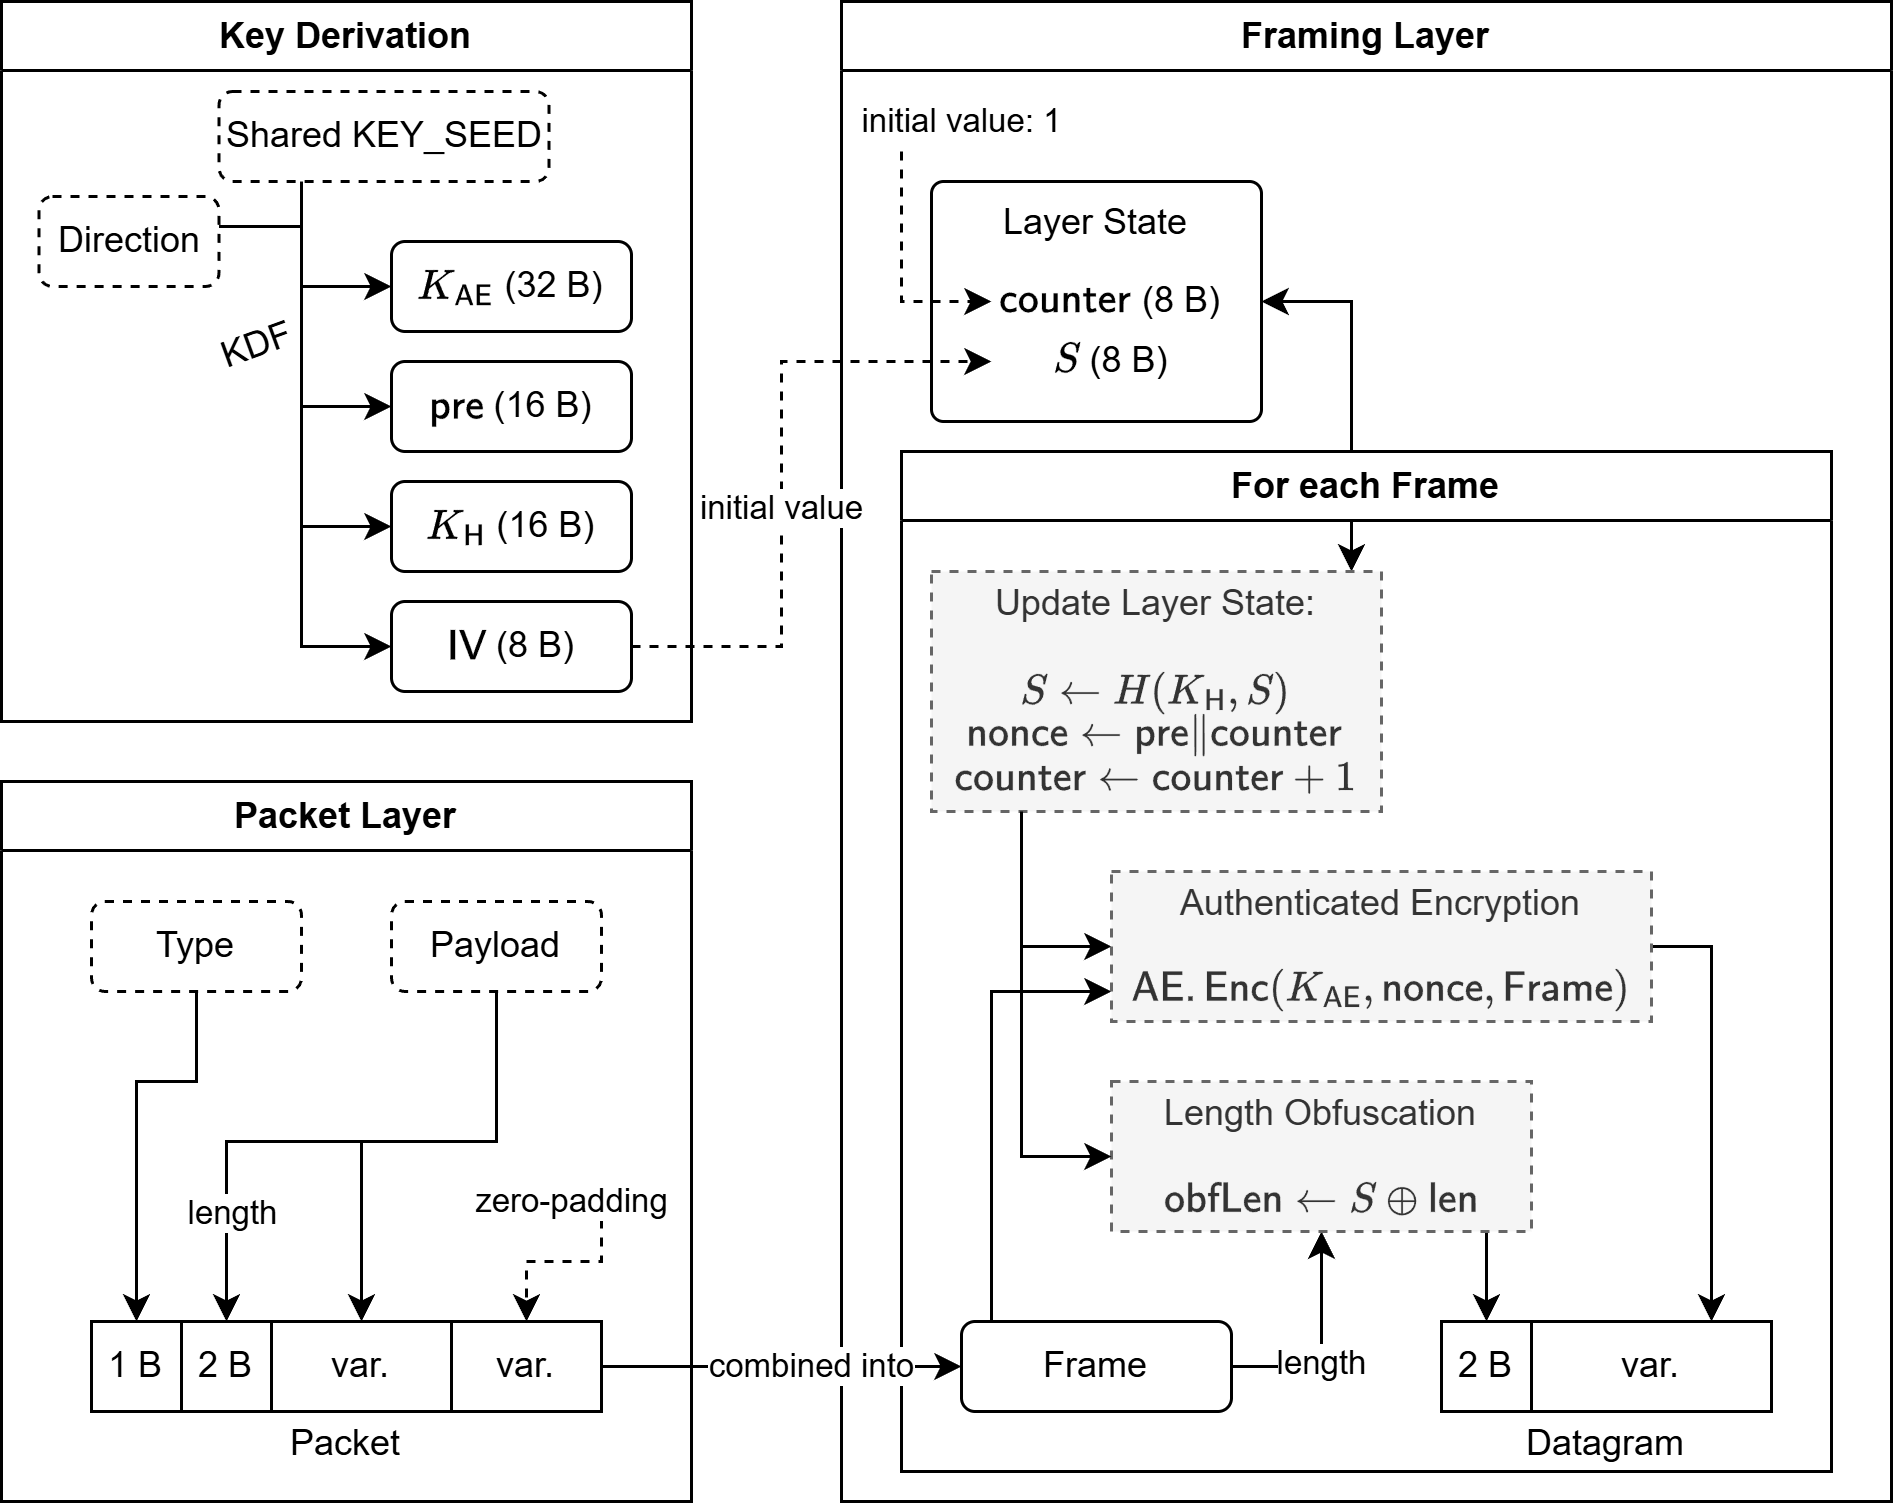
\includegraphics[width=\linewidth]{images/packet-framing.drawio.png}
    \caption[
        A visualization of \obfsfour{} framing at the sender.
    ]{
        A visualization of \obfsfour{} framing at the sender, where dashed shaded boxes correspond to subroutines, dashed unshaded boxes denote inputs, $\mathsf{AE}$ denotes the NaCl secretbox authenticated encryption scheme, and $H$ denotes the SipHash-2-4 pseudorandom function.
    }
    \label{fig:framing}
\end{figure}

To create a packet, a packet type and the payload are required. The packet is then constructed and consists of the following:
\begin{itemize}
    \item A 1-byte packet type (corresponding to ``Payload'' or ``PrngSeed''),
    \item a 2-byte payload length in big endian format,
    \item the payload data itself, and
    \item configurable amounts of zero-padding (not included in the length calculation).
\end{itemize}

This packet is then passed on to a framing layer. While the packet layer ensures that a reliably received data stream can be decoded into separate variable-length messages with associated types, the framing layer's job is to encrypt, authenticate, and obfuscate the data.

For each direction, a counter value $\mathsf{counter}$ is initially set to 1, and a hash state $S$ is initialized to $\mathsf{IV}$.

For each frame (consisting of one or more packets) passed to the framing layer, several things occur:
\begin{enumerate}
    \item A nonce is computed as $ \mathsf{pre} \conc \mathsf{counter}$, and $\mathsf{counter}$ is incremented.
    \item One step of SipHash-2-4 in OFB mode is computed, yielding a fresh 8-byte hash state $S \gets H(K_\mathsf{H}, S)$.
\end{enumerate}

The entire packet is then encrypted using NaCl secretbox (Poly1305/XSalsa20) authenticated encryption with key $K_\mathsf{AE}$, producing a ciphertext; note that the ciphertext is longer than the packet payload, as padding and the secretbox overhead are now included.

The length of the ciphertext is then XORed with the first two bytes of the newly computed state $S$. The final datagram consists of:
\begin{itemize}
    \item A 2-byte obfuscated length field, and
    \item the AE ciphertext.
\end{itemize}

Upon receiving a packet, the receiver updates its $\mathsf{counter}$ and $S$ values, deobfuscated the length field, and decrypts the AE ciphertext. Finally, the data is passed up to the packet layer.

\paragraph{An Informal Security Analysis}

We will now discuss the achieved security guarantees by the above approach, to quickly survey possible improvements in future implementations.

The framing layer outlined above cannot, by design of the underlying Tor pluggable transport implementation, hide the length of transmitted frames from active attackers.
After the initial handshake, the connection is ``wrapped'' in the packet and framing layers, and for as long as the connections stay alive, data is passed back and forth between the local Tor client (in plaintext) and the bridge connection (encoded in packets).
If, at any point, a connection closes or raises an error (e.g. because a tag in the framing layer's AE ciphertext failed to verify), the connection is immediately closed, and a TCP FIN packet is sent by the OS as part of closing the TCP file descriptor.
This allows active attackers to choose any TCP burst after the initial handshake, leave the length field in the first two bytes unmodified, arbitrarily change the third byte (part of the 16 byte NaCl secretbox tag, ensuring a decryption failure later), and then slowly send one byte at a time. As the pluggable transport, after reading a valid length value, will wait for all data to arrive, and then verify the AE ciphertext, the total length of the AE ciphertext can be deduced by observing when the connection is closed.

This contrasts harshly with the handling of errors and invalid MAC values in the handshake procedure: There, a random delay between 1 and 60 seconds from the start of the connection is chosen as a deadline, and if a client causes an error in the handshake or does not send enough data in the first 30 seconds, the connection is closed only at this randomized deadline.

If active attackers attempt to fingerprint the connection by modifying the length value to provoke a closure of the connection (e.g. flipping the most significant bit, ensuring an invalid length), the length value is instead chosen as a random valid length between 16 to 1446 bytes. As the connection then remains blocked until the corresponding amount of AE ciphertext is received before the connection is closed, this attack cannot provoke a closure after a fixed, identifiable amount of data. The concept of ``secure closures'' of channels in general is discussed in more detail in \cite{CCS:FenJoh24}.

The main purpose of the length field obfuscation is therefore not to hide it from active attackers, or protect against manipulation (this is done by the authenticated encryption), but instead to make the protocol harder to identify. To this end, it is not clear to us, why $S$ is not instead chosen as e.g.~$S \gets H(K_H, \mathsf{counter})$ to obtain a similarly secure random value to use in the XOR operation. This would remove the need for $\mathsf{IV}, S$ altogether and streamline the construction. Additionally, the \drivel{} PRF $F_1$ could be reused, reducing the number of primitives required in the protocol.

\paragraph{Design Conflicts and Conclusion}

To construct a system capable of flexible traffic shaping, it is necessary to split large messages into smaller ones, sent in sequence, as well as to pad small messages to a larger size, or even send only padding when no message is available.

The existing packet-based system in \obfsfour{} achieves exactly this, while providing authentication and side-stepping attacks from \cite{SP:AlbPatWat09}. Each packet incurs an overhead of 3 bytes plus configurable padding, and each frame (containing one or more packets, depending on the bridge configuration) adds 18 bytes.
The only precondition is a securely shared $\mathsf{KEY\_SEED}$.

It is possible to employ this system directly in \drivel{} (possibly changing the employed schemes in the framing layer to match KEM and OKEM security levels).
For example, we could first transmit $c_S \conc A_C$ without using the framing layer, and then initialize the framing layer using a key derived from the early secret $ES$. Later, we could re-initialize the framing layer using yet another key after the handshake is completed.

However, since the framing layer already aims to provide obfuscation, integrity, and confidentiality, the need for $P_C, M_C, \mathsf{MAC}_C, P_S, M_S, \mathsf{MAC}_S$ would disappear. Note that the message transcript is implicitly validated by including the $\mathsf{context}$ value when calculating $\mathsf{KEY\_SEED}$. Furthermore, it would not be necessary to encrypt $\pk_e$ at all.

We believe it to be worthwhile to modify \drivel{} accordingly, allowing almost arbitrary traffic shaping after an initial transmission of only $c_S \conc A_C$.
Conversely, this rather extensive change would require adapting the extensive $\sObfKE$ security proof for \drivel{} presented in \cite{EPRINT:GRSV25}.

This approach is visualized in \cref{fig:modified-drivel-framing}, an adaptation of \cref{fig:drivel}. Let $FL$ denote the framing layer presented above. Then $FL.\mathsf{Rekey}(k)$ indicates that the framing layer is reinitialized using $k$ as the $\mathsf{KEY\_SEED}$ value following the process outlined above.

In addition, we took the opportunity to propose a simplification of the calculation of PRF values in order to optimize memory performance:
As $F_1$ is implemented as \textsf{HDKF-Expand}, its state after digesting part of its input cannot be reused for further calls to $F_1$ (due to e.g. the string constants used for domain separation) and its entire input must be re-hashed when requesting multiple output blocks.
Both shortcomings can be circumvented by instead pre-hashing long inputs without appending a string constant. This hash state could also be reused when more inputs are desired in the later stages of the protocol.

To this end, we introduce a hash function $\mathbf{H}$ and replace the inputs to $F_1$ appropriately. This approach is similar in spirit to e.g. the calculation of the transcript hash in TLS 1.3 by keeping a running hash value \cite[Section~4.4.1]{rfc8446}.

\begin{figure}
    % \begin{minipage}[t]{\textwidth}
	\hfill
	\pseudocode[codesize=\footnotesize,jot=-1mm]{%
		\textbf{Server key generation/setup} \\
		\nodeid \getsr \bin^{\nodeidlen} \\
		(\pk_S, \sk_S) \getsr \OKEM.\kgen() \\
		\pstate.\macregister \gets \emptyset \\
		\text{return } ((\pk_S, \nodeid), (\sk_S, \nodeid), \pstate)
	}
	\hspace*{0.8cm}
% \end{minipage}

% \vspace{0.5em}

% \hspace*{-0.2in}
\centering
\scalebox{0.9}{%
\begin{tikzpicture}
	% Set the X coordinates of the client, server, and arrows
	\edef\ClientX{0}

	\edef\ArrowLeft{3}
	\edef\ArrowRight{13}
	\edef\ServerX{16.5}
	\edef\ServerLeftTextwidth{10.5cm} % width of server-side text, when left-aligned

	% Set the starting Y coordinate
	\edef\Y{0}

	% Draw header boxes
	\node [rectangle,draw,inner sep=5pt,right] at (\ClientX,\Y) {\textbf{Client}};
	\node [rectangle,draw,inner sep=5pt,left] at (\ServerX,\Y) {\textbf{Server}};
	
	\NextLine[0.4]
	\ClientAction[gray,font=\small]{\hspace{1.5cm}knows $(\pk_S, \nodeid)$}
	\ServerAction[gray,font=\small]{knows $(\sk_S, \nodeid)$\hspace{1.5cm}\null}
	\NextLine[1.1]
	
	\ClientAction{$(\pk_e, \sk_e) \getsr \KEM.\kgen()$} 
	\NextLine
	\ClientAction{$(c_S, K_S) \getsr \OKEM.\encaps(\pk_S)$}
	\NextLine
	\ClientAction{$ES \gets \funComb(\nodeid, K_S)$}
	\NextLine
	\ClientAction{$\mathsf{protoID} \gets \textlit{Drivel}$}
	\NextLine
	\ClientAction{\highlightbox{$\mathsf{context}_1 \gets \mathsf{protoID} \conc \pk_S \conc c_S$}}
	\NextLine
	\ClientAction{\highlightbox{$A_C \gets \funPRF(ES, \mathbf{H}(\mathsf{context}_1) \conc \textlit{:authc})$}}
	\NextLine
	\ClientAction{\highlightbox{$\mathsf{KEY\_SEED}_1 \gets \funPRF(ES, \mathbf{H}(\mathsf{context}_1) \| \textlit{:key\_extract\_1})$}}
	%%%%%%%%%%%%%%%%%%%%%%%%%%%%%%%%%%%%%%%%%%%%%%%%%%%%%%%%%%%%%%%%%%%%%%%%%%%%%%%%%%%%%%%%%%%%%%%%%%%%%%%
	\NextLine[2]
	\ClientToServer{\highlightbox{$\mathsf{msg}_C' = c_S \conc A_C$}}{}
	\NextLine
    %%%%%%%%%%%%%%%%%%%%%%%%%%%%%%%%%%%%%%%%%%%%%%%%%%%%%%%%%%%%%%%%%%%%%%%%%%%%%%%%%%%%%%%%%%%%%%%%%%%%%%%

    % Server verifies A_C and can start with dummy data
	\ServerActionLeft{$K_S \gets \OKEM.\decaps(\sk_S, c_S)$}
	\NextLine
	\ServerActionLeft{$ES \gets \funComb(\nodeid, K_S)$}
	\NextLine
	\ServerActionLeft{$\mathsf{protoID} \gets \textlit{Drivel}$}
	\NextLine
	\ServerActionLeft{\highlightbox{$\mathsf{context}_1 \gets \mathsf{protoID} \conc \pk_S \conc c_S$}}
	\NextLine
	\ServerActionLeft{\highlightbox{if $\funPRF(ES, \mathbf{H}(\mathsf{context}_1) \conc \textlit{:authc}) \neq A_C$: $\texttt{break}$}}
	\NextLine
	\ServerActionLeft{if \highlightbox{$A_C$}$ \in \pstate.\macregister$: $\texttt{break}$}
	\NextLine
	\ServerActionLeft{$\pstate.\macregister \gets \pstate.\macregister \cup $\highlightbox{$\{A_C\}$}}
	\NextLine
	\ServerActionLeft{\highlightbox{$\mathsf{KEY\_SEED}_1 \gets \funPRF(ES, \mathbf{H}(\mathsf{context}_1) \| \textlit{:key\_extract\_1})$}}
    %%%%%%%%%%%%%%%%%%%%%%%%%%%%%%%%%%%%%%%%%%%%%%%%%%%%%%%%%%%%%%%%%%%%%%%%%%%%%%%%%%%%%%%%%%%%%%%%%%%%%%%

    % Rekeying 1
    \NextLine
	\PhaseBreak{}{}
	\NextLine
    \ClientAction{\highlightbox{$FL.\mathsf{Rekey}(\mathsf{KEY\_SEED}_1)$}}
    \ServerAction{\highlightbox{$FL.\mathsf{Rekey}(\mathsf{KEY\_SEED}_1)$}}
    \NextLine[0.5]
	%%%%%%%%%%%%%%%%%%%%%%%%%%%%%%%%%%%%%%%%%%%%%%%%%%%%%%%%%%%%%%%%%%%%%%%%%%%%%%%%%%%%%%%%%%%%%%%%%%%%%%%

    % Start sending arbitrary data
	\ServerToClient[dashed,->]{}{}
	\ServerAction{\highlightbox{send arbitrary data}}
    %%%%%%%%%%%%%%%%%%%%%%%%%%%%%%%%%%%%%%%%%%%%%%%%%%%%%%%%%%%%%%%%%%%%%%%%%%%%%%%%%%%%%%%%%%%%%%%%%%%%%%%
    \NextLine[2]
	\ClientToServer{\highlightbox{$\mathsf{msg}_C'' = \pk_e$}}{}
	\NextLine
	%%%%%%%%%%%%%%%%%%%%%%%%%%%%%%%%%%%%%%%%%%%%%%%%%%%%%%%%%%%%%%%%%%%%%%%%%%%%%%%%%%%%%%%%%%%%%%%%%%%%%%%

    % Server parses rest of message and replies
    \ServerActionLeft{$(c_e, K_e) \getsr \KEM.\encaps(\pk_e)$}
	\NextLine
	\ServerActionLeft{$ES' \gets \funPRF(ES, \textlit{:derive\_key})$ ; $FS \gets \funComb(ES', K_e)$}
	\NextLine
	\ServerActionLeft{\highlightbox{$\mathsf{context}_2 \gets \mathsf{context}_1 \conc \pk_e \conc c_e$}}
	\NextLine
	\ServerActionLeft{$\mathsf{KEY\_SEED}_2 \gets \funPRF(FS, $\highlightbox{$\mathbf{H}(\mathsf{context}_2)$}$ \conc \textlit{:key\_extract\_2})$}
	\NextLine
	\ServerActionLeft{$\mathsf{auth} \gets \funPRF(FS, $\highlightbox{$\mathbf{H}(\mathsf{context}_2)$}$ \conc \textlit{:server\_mac})$}
	%%%%%%%%%%%%%%%%%%%%%%%%%%%%%%%%%%%%%%%%%%%%%%%%%%%%%%%%%%%%%%%%%%%%%%%%%%%%%%%%%%%%%%%%%%%%%%%%%%%%%%%
	\NextLine[1.5]
	\ServerToClient{\highlightbox{$\mathsf{msg}_S = c_e \conc \mathsf{auth}$}}{}
    %%%%%%%%%%%%%%%%%%%%%%%%%%%%%%%%%%%%%%%%%%%%%%%%%%%%%%%%%%%%%%%%%%%%%%%%%%%%%%%%%%%%%%%%%%%%%%%%%%%%%%%

    \NextLine
	\ClientAction{$K_e \gets \KEM.\decaps(\sk_e, c_e)$}
	\NextLine
	\ClientAction{$\mathsf{protoID} \gets \textlit{Drivel}$}
	\NextLine
	\ClientAction{$ES' \gets \funPRF(ES, \textlit{:derive\_key})$ ; $FS \gets \funComb(ES', K_e)$}
	\NextLine
	\ClientAction{\highlightbox{$\mathsf{context}_2 \gets \mathsf{context}_1 \conc \pk_e \conc c_e$}}
	\NextLine
	\ClientAction{$\mathsf{KEY\_SEED}_2 \gets \funPRF(FS, $\highlightbox{$\mathbf{H}(\mathsf{context}_2)$}$ \| \textlit{:key\_extract\_2})$}
	\NextLine
	\ClientAction{if $\funPRF(FS, $\highlightbox{$\mathbf{H}(\mathsf{context}_2)$}$ \conc \textlit{:server\_mac}) \neq \mathsf{auth}$: $\texttt{break}$}
    %%%%%%%%%%%%%%%%%%%%%%%%%%%%%%%%%%%%%%%%%%%%%%%%%%%%%%%%%%%%%%%%%%%%%%%%%%%%%%%%%%%%%%%%%%%%%%%%%%%%%%%

    % Rekeying 2
    \NextLine
	\PhaseBreak{}{}
	\NextLine
    \ClientAction{\highlightbox{$FL.\mathsf{Rekey}(\mathsf{KEY\_SEED}_2)$}}
    \ServerAction{\highlightbox{$FL.\mathsf{Rekey}(\mathsf{KEY\_SEED}_2)$}}
\end{tikzpicture}
}

    \caption[
        The modified \drivel{} protocol, simplified to take advantage of a framing layer.
    ]{
        The modified \drivel{} protocol, simplified to take advantage of a framing layer.
        $\OKEM$ is an OKEM satisfying $\indcca, \sprcca$ security, and ciphertext uniformity.
        $KEM$ is an $\indonecca$-secure KEM.
        $FL$ is a framing layer similar to the one described in \cref{sssec:variant-framing}.
        $F_1$ is a PRF and $F_2$ is a dual PRF.
        $\mathbf{H}$ is a collision-resistant hash function.
        Core differences to the \drivel{} protocol from \cref{fig:drivel} are highlighted in blue boxes.
        Messages are easily parsed due the the packet layer providing boundaries and the fixed-length components.
        A dashed arrow represents the option to send an arbitrary amount of uniformly random bits for the purpose of traffic shaping, e.g. by sending packets consisting only of padding.
        Dotted lines delimit the framing layer phases between $FL.\mathsf{Rekey}$ operations.
    }
    \label{fig:modified-drivel-framing}
\end{figure}

\paragraph{Note to Implementers and Future Work}

Should readers choose to implement or improve upon this proposed variant of \drivel{}, we encourage them to also consider the following items:

\begin{itemize}
    \item Calculating $\mathbf{H}(\mathsf{context}_2)$ can be done efficiently by reusing the hash state after digesting $\mathsf{context}_1$, avoiding the need to hash $\mathsf{context}_1$ twice. The hash outputs can be reused for two invocations of $F_1$ each time.
    
    \item This variant does not have a security proof like \drivel{}, and producing one would require formalizing the guarantees provided by the framing layer.

    \item As this thesis focuses on the key exchange phase, we did not propose improvements to the framing layer. However, previous work in this space exists \cite{CCS:FenJoh24} and should be considered to improve the framing layer from \obfsfour{}.

    \item Attention should be paid in particular to preventing modifications to the length fields (e.g. by authenticating them using fixed-length fields), and to handling errors consistently as discussed in the security analysis above and in \cite[Section~3.3]{CCS:FenJoh24}.

\end{itemize}

